\chapter{State-of-the-Art} \label{chap:sota}

\section*{}

In this chapter we will begin by making a more in depth presentation of the
process of gene expression. This will be followed by a literature and state of
the art review in the fields of genome/\trans{} assembly and data mining.
Lastly, we will present some of the tools used in each of those areas, as well
as some relevant data representation formats for genetic data.

\section{Biological Base Concepts}

Before dwelling in the details of the state of the art that are on the
foundation of this thesis, it is important to explain some concepts of the
domain of molecular biology. As explained in Section \ref{sec:context}, gene
expression is the mechanism by which an organism's \dna{} can be expressed into
functional genetic products, like proteins, rRNA and tRNA. This process starts
with the genetic code, or nucleotide sequence, of each gene. Different genes in
an organism's \dna{} are responsible for the creation of different genetic
products. The process of gene expression itself is composed by two main stages,
transcription and translation \cite{leic:gene_expr}.

Transcription is the stage at which genetic data in the form of \dna{} is used
to synthesize \rna{}, being this the process that concerns the thesis main
question. Several different types of \rna{} are produced by this process,
including mRNA (which specifies the sequences of amino acids that form a
protein), rRNA and tRNA, both later used in the translation stage. Simplifying a
gene's structure, it can be seen as composed by two types of areas, introns and
exons, as seen in Figure \ref{fig:intron_exon}.

\begin{figure}[!htb]
  \begin{center}
    \leavevmode
    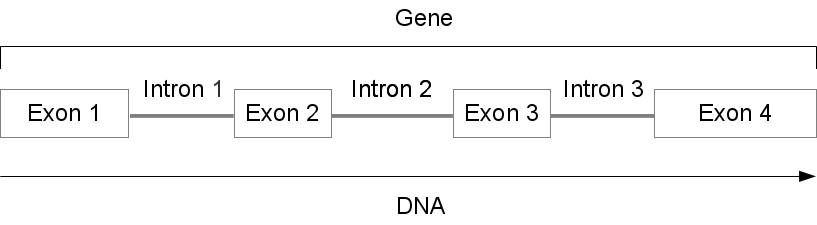
\includegraphics[width=0.7\textwidth]{intron_exon}
    \caption{Overall structure of a gene, with its different areas (simplified)}
    \label{fig:intron_exon}
  \end{center}
\end{figure}

Only the exons are useful in the gene expression process, being also known as
coding regions. Introns, on the other hand, are not used in the process. They
are present in an early stage mRNA molecule, the precursor RNA, but are later
removed (or spliced) in the final molecule before the translation stage
\cite{leic:gene_expr}. Figure \ref{fig:splicing} illustrates the removal of
introns from the mRNA molecule, during the  splicing process. As stated before,
the main goal of this thesis is to explain how the final nucleotide sequence of
each exon affects the transcription speed of the exon itself.

\begin{figure}[!htb]
  \begin{center}
    \leavevmode
    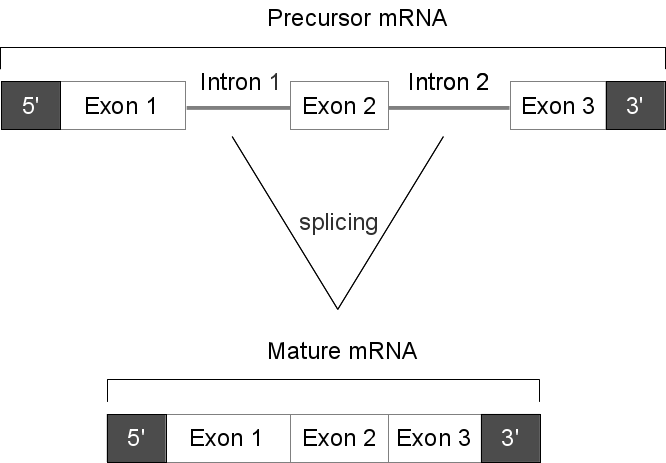
\includegraphics[width=0.58\textwidth]{splicing}
    \caption{The removal (splicing) of introns from the precursor mRNA, during
    the transcription process}
    \label{fig:splicing}
  \end{center}
\end{figure}

After the conclusion of the transcription process comes the translation process.
In this process, the synthesized mRNA is used to specify the sequence of amino
acids that constitute the particular protein being produced. The other types of
RNA molecules (rRNA and tRNA) are also used in this stage of the gene expression
process.

Obtaining this genetic information is done experimentally, by employing a genome
sequencing technique. For quite some time this process was carried out using the
Sanger sequencing method and other similar methods \cite{Reis-Filho2009}. Though
effective, such methods we're notably slow and costly, with large projects like
the Human Genome Project (HGP) consuming roughly thirteen years and US\$ 3
billion. Other than the realm of human genetics, this kind of study was
restricted to model organisms, such as the fruit fly and mouse genomes
\cite{Wolf2013}. The past few years have seen the appearance and rise in
popularity of the \ngs{} techniques. These techniques differ from the more
classical ones by producing larger amounts of information, in less time. They
are also typically more cost effective than previous techniques and can be
easily employed by single laboratories, which has greatly contributed to their
popularity. As a disadvantage, \ngs{} techniques produce shorter reads than
their older counterparts, being that \qt{\textit{(...) transcriptome assembly
from billions of RNA-Seq reads (...) poses a significant informatics challenge}}
\cite[p. 671]{Martin2011} Although this thesis will not deal with the problems
of sequencing techniques, it is important to indicate that the read dataset that
will be used is a result of \ngs{} techniques. As such, we will use assembly
techniques more suited to situations where short reads are available.

\section{\rnaseq{} and \Trans{} Assembly}\label{sec:assembly}

\Trans{} assembly is the process by which experimentally obtained genetic data
reads can be organized and merged together in a partial or complete genome
expression profile. As stated above, the advent of next generation sequencing
techniques, with their reduced costs, greatly increased the availability of
genome sequencing data.

For years, microarrays were the standard tool available for examining features
of the transcriptome and global patterns of gene expression \cite{Wolf2013}.
However, microarrays typically produce data more oriented towards assembly
against existing reference data, hence limiting its application to species with
well known reference genomes. This is impractical, as \ngs{} techniques allow to
cheaply obtain genetic information of previously not studied species. This is
one of the reasons that led to the inception of RNA-Seq. Contrary to
microarrays, RNA-Seq techniques are able to wield results that are suitable for
both reference guided assembly and \textit{de novo} assembly approaches
\cite{Wilhelm2009}. \textit{De novo} or exploratory assembly has captured the
interest of researchers in the past few years, leading to the appearance of
multiple RNA-Seq tools that are capable of making this type of assembly without
a reference genome \cite{nuno11:assemblathon}. Despite this amazing capability,
we will restrict this project to reference genome guided problems, which are
simpler and more oriented to a Masters level thesis.

\subsection{\rnaseq{} Tools}\label{sec:seqtools}

Below we will present some bioinformatic tools, used to support the multiple
steps of the RNA-Seq process. Although there are several tools capable of
executing all steps of the RNA-Seq process, it has been decided that in this
project we will create our own assembly pipeline, using specialized tools for
every step. We will also present some of the most popular file formats used in
this context, along with some tools used to manipulate these files.

\subsubsection*{Tuxedo Suite}

% TODO

\paragraph{TopHat}

% TODO

\paragraph{Bowtie}

% TODO

\paragraph{Cufflinks}

% TODO

\paragraph{CummeRbund}

% TODO

\subsubsection*{Burrows-Wheeler Aligner}

% TODO

\subsubsection*{SAM Tools}

% TODO

\subsubsection*{BLAST}

% TODO

\subsection{Relevant Standard File Formats}\label{sec:formats}

As expected, the great diversity of \rnaseq{} tools brings with it a wealth of
file formats. Some of these formats are developed from the ground up to satisfy
a specific need, while other are mere contextual adaptations or specializations
of already established formats. Below we will present a few of the most popular
and wide spread file formats, talking about their basic structure, the types of
data they represent and their applications.

\subsubsection*{FASTA}

FASTA is the standard line and character sequence format used by NCBI
\cite{ncbi:fasta}, using this last organization's character code conventions. It
is a simple format, that can be used to easily store data represented by
character sequences, like nucleotide (\dna, \rna) or amino acid (protein)
sequences. This file format is widely use to store sequencing reads, \dna/\rna{}
sequences and other character sequences in database systems. Its simplicity
makes it extremely easy to manipulate and parse, presenting also an attractive
solution for data transfer between different tools.

\subsubsection*{FASTQ}

FASTQ is used to store store character sequences, typically nucleotide sequences
\cite{Cock2010}. It's quite similar to the standard FASTA format, in respect to
the manner in which character sequences are represented. However, for every
sequence, there is a second sequence of equal length, representing the quality
scores of the original sequence. These quality scores are also represented as
single characters, taking values between and including ASCII-33 to ASCII-126.
It's typically used in the same situations as the FASTA format, when quality
scores are available/relevant.

\subsubsection*{SAM and BAM}

The SAM format is a text format for storing sequence alignment data
\cite{genome:sam}. It is widely used to store mapping information between
sequencing reads and a given reference genome. This sort of information is
typically the product of sequencing alignment tools, that consume sequencing
reads from FASTQ files and align them with a reference genome.

The BAM format contains exactly the same information as the SAM format and the
same rules apply for both formats. The difference between both formats lies in
their encoding. While SAM is a text based format, BAM is a binary format. This
means that BAM sacrifices human readability for increased machine processing
performance, as it is more efficient to work with compressed and indexed binary
data.

\subsubsection*{VCF}

VCF is a text file format used to store gene sequence variants \cite{smith13}.
In the past few years, as larger and larger \dna{} sequencing projects became
more common (like the 1000 Genomes Project\footnote{The 1000 Genomes Project,
started back in 2008, is an international effort to establish the most
comprehensive catalogue to date of human genetic variations.}), storing such
large amounts of information became a serious concern. To address these concerns
the VCF format was created. Instead of storing the complete genome, VCF stores
only the variations (and their respective positions) of newly sequenced genomes
relatively to a known reference genome, typically in a compressed text file. As
such, it is a format often used when building genome databases.

\subsubsection*{GFF and GTF}

GFF is a text based file format to store gene features \cite{sanger11}. Many
genome assembly tools execute this process in two seperate steps: feature
detection for identification of specific regions (exons, introns, etc.) and
genome assembly, using those features as reference. However, often times it is
beneficial to decouple these two steps, using different and more efficient tools
for each. As such, the GFF format emerged as a protocol for feature information
transfer between tools.

The GTF format is similar to the GFF format, in which it is based. It is also
used in similar situations. However, GTF builds on top of GFF, defining
additional conventions, specific to the domain of genetic information. Despite
their initial relation, both formats are developed individually.

\section{Data Mining}\label{sec:mlearning}

Data mining is the process of \qt{\textit{extracting or \qt{mining} knowledge
from large amounts of data}} \cite[p. 5]{han2006data}. As such, it consists in a
set of techniques that can be used to find interesting patterns in large data
sets, that translate in newfound knowledge. Data mining borrows techniques from
multiple fields, such as artificial intelligence, machine learning, statistics,
and database systems \cite{Chakrabarti2012}. Its ultimate goal is to combine all
those techniques and transform large and (apparently) meaningless sets of data
into understandable and useful information. Thus, data mining was motivated by
the perspective of harnessing the abundance of data, that characterizes today's
information systems, to produce meaningful knowledge.

Because of their large quantities of input data, data mining tasks are usually
totally, or at least partially, automated. As such, there are several algorithms
for these tasks and tools that implements such algorithms, as presented in
Section \ref{sec:minalgo} and Section \ref{sec:mintools}, respectively.

We can divide data mining into main types: descriptive data mining and
predictive data mining \cite{Fayyad1996}. Descriptive data mining is focused on
finding the underlaying structure of a given set of data. Instead of predicting
future values, it concerns the intrinsic structure, relations and
interconnectedness of the data being analysed, presenting its interesting
characteristics without having any predefined target. On the other hand,
predictive data mining is used to predict explicit values, based on patterns
determined from the dataset. With predictive data mining we try to build models
using known data and use those models as a base to predict future behaviour.

As we're seeing, data mining does not represent a single type problem. In fact
there are several different types of problems that can be addressed by data
mining techniques. Each of these problems may require a different data mining
method. A brief review of the most common methods is given below.

\begin{description}

  \item[Classification]
  is a method that tries to generalize the already known structure, so that it
  applies to new datasets. In other words, with classification we try to learn a
  function that is capable of mapping our data into predefined classes.

  \item[Regression]
  tries to learn a function that models relationships between variables in the
  dataset. That function can latter be used to find real value predictions of
  future behaviour of the same or similar datasets.

  \item[Clustering]
  consists in identifying a finite set of categories or clusters of similar
  values, to describe the dataset. As such, it is used without prior knowledge
  about data structure.

  \item[Summarization]
  provides a more compact representation of a subset of data, in a way that the
  summarized data retains the central points of the original data. This can be
  accomplished in several different ways, like using report generation or
  multivariate visualization techniques.

  \item[Dependency modelling]
  finds a model which describes relationships between variables, revealing their
  dependencies.

  \item[Change and deviation detection]
  tries to discover the most significant changes in the data, when compared with
  previously measured data. This method is useful to find interesting data
  variations or data errors.

\end{description}

\subsection{Data Mining Algorithms}\label{sec:minalgo}

In this project we will be concerned with the classification side of data
mining. Below, we will review some algorithms that can be used in
classification problems.

\subsubsection*{Decision Trees}

% TODO

\subsubsection*{Random Forest}

% TODO

\subsubsection*{Support Vector Machines}

% TODO

\subsubsection*{K-NN}

% TODO

\subsubsection*{Inductive Logic Programming}

% TODO

\subsection{Model Evaluation Procedures and Measures}

Creating a data model using a suitable classification algorithms is not the last
step in the data mining process. At this point our model works well with the
original training data, but we need to verify its power to generalize to other
sets of data. Without this evaluation process, our models may be susceptible to
problems like overfitting, in which the model wrongly describes a random error
or data noise as a significant pattern \cite{han2006data}. As such, we need
methods that allow us to test our models before deployment, as well as standard
measures, to determine their quality.

\subsubsection*{Evaluation Procedures}

As stated, evaluation procedures are essential to verify the generalization
capabilities of a given model. These procedures typically consist of dividing
the test dataset in two or more subsets, using some of them for training and the
others for testing. We will present a brief overview of some of these procedures
below.

\paragraph{Hold-Out}

The \textit{hold-out} method reserves a part of the dataset for training
purposes and uses the remaining data for testing \cite{witten2011data}.
Typically we separate one third of the original dataset for testing, using the
other two thirds for training.

However, this arbitrary division of the dataset might be problematic if the
subsets aren't representative of the population. For example, if the test subset
is missing a class our results might be erratic. One way to attenuate this
problem is to use stratification. Using stratification of the dataset we ensure
that both subsets are representative, with approximately equal proportions for
each class. We can lessen error rates even further and make the
\textit{hold-out} estimate more reliable using the \textit{repeated hold-out}
method. This is an iterative method, where in each iteration a subset is
randomly selected to use as training (possibly using set stratification), using
the remaining subset for testing. After all the iterations, the error rates of
each one are averaged to yield an overall error rate.

\paragraph{Cross-Validation}

\textit{Repeated hold-out} methods pose a problem: the different test subsets
will eventually overlap. This may cause that some examples never appear in the
training subsets. The overlapping problem can be solved using the
\textit{cross-validation} procedure, also called \textit{k-fold
cross-validation}. This method consists in splitting the original dataset into
\textit{k} subsets, using each subset in turn for testing and the remainder for
training.

The standard method for evaluation is \textit{10-fold cross validation}, where
the dataset is divided into ten subsets. The subsets are typically stratified to
reduce result variance. In each iteration one of the ten folds is picked as test
and the other nine are used for training. Sometimes, to further reduce variance,
\textit{repeated stratified cross-validation} is used, repeating normal
\textit{10-fold cross-validation} ten times, then averaging the results.

\paragraph{Leave-One-Out}

\textit{Leave-one-out} method is a form of \textit{cross-validation}, taken to
extreme lengths. In this particular method, the original dataset is divided into
\textit{n} folds, where \textit{n} is the number is the number of individual
training instances. It has some benefits, like allowing for a better use of the
dataset and involving no random set sampling. However, the sheer number of folds
and tests makes it a very computationally expensive method. Another disadvantage
is that no stratification is possible, as there is always only one instance in
the test subset.

\subsubsection*{Common Measures}

% TODO

\paragraph{Accuracy}

% TODO

\paragraph{Precision}

% TODO

\paragraph{Recall}

% TODO

\paragraph{F-Measure}

% TODO

\paragraph{AUC}

% TODO

\subsection{Data Mining Tools}\label{sec:mintools}

Except in rare cases of very specific problems, it typically makes no sense for
someone to implement any data mining algorithm that they might need. In fact,
today we have lots of data mining tools (many of which are free), that already
implement many of those algorithms. These tools are usually customizable, making
it easy to adapt them to most problems. Below we'll briefly review some of the
most popular data mining tools, that apply to the specific needs of this thesis.

\subsubsection*{RapidMiner}

RapidMiner\footnote{\url{http://www.rapidminer.com/}} is a complete solution for
data mining problems. It's available as a standalone GUI based application, as
seen in Figure \ref{fig:rapidminer}. It is a commercial application, although
its core and earlier versions are distributed under an open source license and
it offers a free version, beyond its multiple paid versions. Being one of the
most popular data mining tools used today, its applications span several
domains, including education, training, industrial and personal applications,
among others. Its functionality can also be easily extended through the use of
plugins\footnote{Plugin is a software module that adds new functionality to an
existing software application. Plugins are typically dependent on the platform
they extend and can't be used as standalone tools.}, reflecting in an increased
value for this tool. One such example in the area of bioinformatics is the
integration plugin between RapidMiner and the
Taverna\footnote{\url{http://www.taverna.org.uk/}} open source workflow
management system \cite{Jupp2011}.

\begin{figure}[!htb]
  \begin{center}
    \leavevmode
    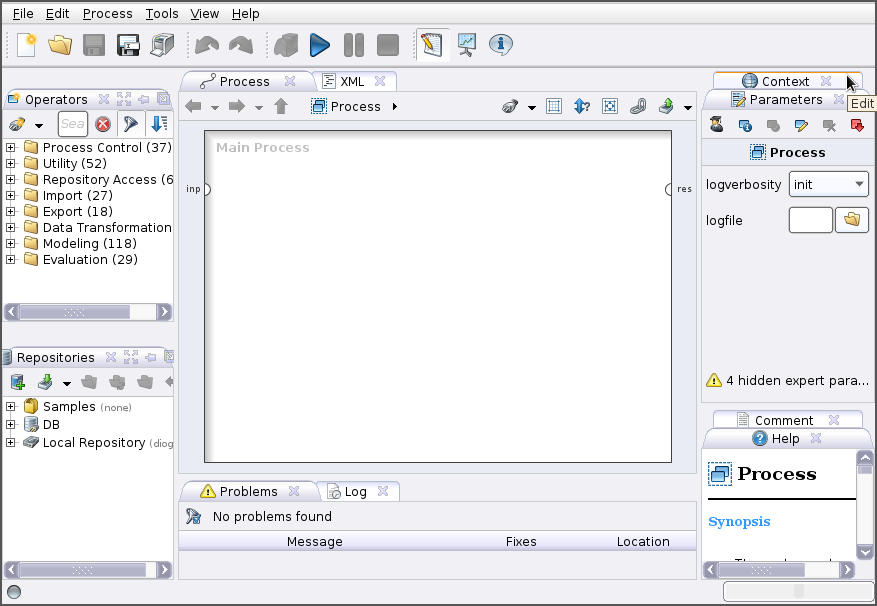
\includegraphics[width=1.0\textwidth]{rapidminer}
    \caption{RapidMiner user interface}
    \label{fig:rapidminer}
  \end{center}
\end{figure}

\subsubsection*{Weka}

Weka\footnote{\url{http://www.cs.waikato.ac.nz/ml/weka/}} is an open source tool that
collects several machine learning algorithms and allows its user to easily apply
those algorithms to data mining tasks \cite{Hall}. Created at the University of
Waikato, New Zeland in 1997 (the current version was completely rewritten in
1997, despite the first iteration of the tool being developed as early as 1993),
it's still in active development to date. Weka supports several common data
mining tasks, like data preprocessing, classification, clustering, regression
and data visualization. It's core libraries are written in Java and allow for an
easy integration of its data mining algorithms in pre existing code and
applications. Other than that, Weka can be used directly through a command
line/terminal or through one of its multiple GUI's (Figure \ref{fig:weka}). Its
simple API and well structure architecture allow it to be easily extended by
users, should they need new functionalities.

\begin{figure}[!htb]
  \begin{center}
    \leavevmode
    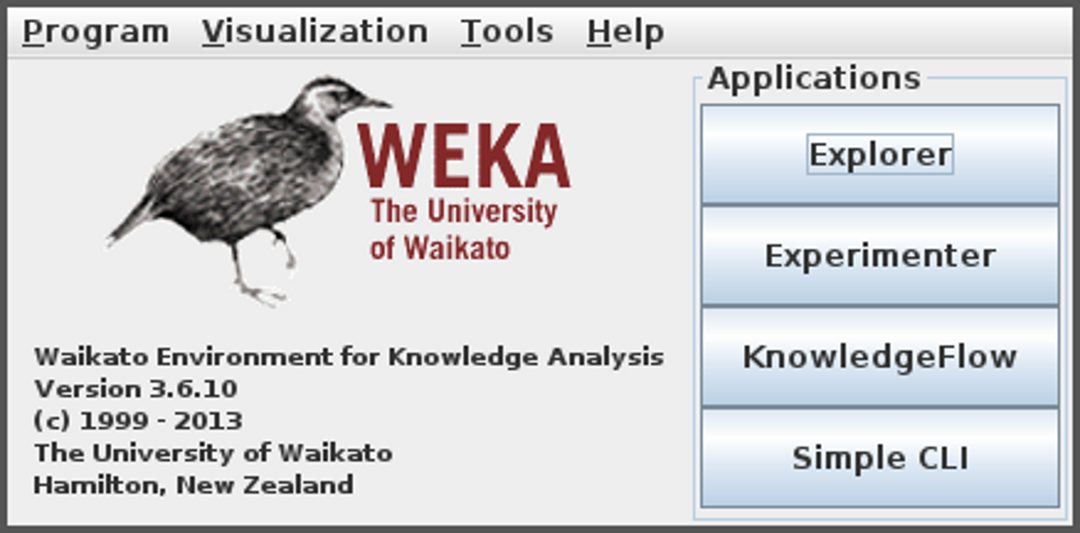
\includegraphics[width=0.7\textwidth]{weka}
    \caption{Weka interface selection}
    \label{fig:weka}
  \end{center}
\end{figure}

\subsubsection*{R Language}

R\footnote{\url{http://www.r-project.org/}} is a free programming language and
software environment for statistical computing and graphics generation.
Originally developed by Ross Ihaka and Robert Gentleman at the University of
Auckland, New Zealand in 1993 \cite{Ihaka1998}, it's still under active
development. R is typically used by statisticians and data miners, either for
direct data analysis or for developing new statistical software \cite{Fox2005}.

R is an implementation of the S programming language\footnote{S is an object
oriented statistical programming language, appearing in 1976 at Bell
Laboratories.}, borrowing some characteristics from the Scheme programming
language. It's core is written in a combination of C, Fortran and R itself. It
is possible directly manipulate R objects in languages like C, C++ and Java. R
can be used directly through the command line or through several third party
graphical user interfaces like
Deducer\footnote{\url{http://www.deducer.org/pmwiki/index.php}}. There are also
R wrappers for several scripting languages.

R provides several different statistical and graphical techniques, including
linear and nonlinear modeling, classical statistical tests, time-series
analysis, classification, clustering, among others. It can also be used to
produce publication-quality static graphics. Tools like Sweave
\cite{lmucs-papers:Leisch:2002} allow users to embed R code in \LaTeX{}
documents, for complete data analysis.

\paragraph{Bioconductor Package}

Bioconductor is a free and open source set of tools for genomic data analysis,
in the context of molecular biology \cite{lmucs-papers:Leisch:2002}. It is
primarily based on R. It is under active development, with two stable releases
each year. Counting with more than seven hundred different packages, it's the
most comprehensive set of genomic data analysis tools available for the R
programming language. It also provides a set of tools to read and manipulate
several of the most common file formats used in molecular biology oriented
applications, including FASTA, FASTQ, BAM and GFF.

\section{Chapter Conclusions}

% TODO

- in this chapter we talked about...\\
- we don't know where classification algorithms will be sufficient or if we'll
  need ILP...\\
- what else?\\
